\documentclass{beamer}
\usetheme{default}
\definecolor{LiUblue}{RGB}{0,185,231}
\usecolortheme[named=LiUblue]{structure}

\title{Quantifying nitrogen oxides and ammonia via frequency modulation in gas sensors}
\subtitle{Master Thesis - Mid term seminar}
\author{Marcos F Mourão}
\date{March 25, 2021}
 
\begin{document}
	\begin{frame}
		\titlepage
	\end{frame}

\begin{frame}
	\frametitle{Outline}
	\tableofcontents
\end{frame}

\begin{frame}
	\section{Problem recap}
	\frametitle{Problem in a nutshell}
	
	\subsection{Motivation}
	NOx are detrimental to the environment
	
	Ammonia can neutralize NOx
	
	Gas sensors can be used to quantify NOx and Ammonia
	
	However, it is not trivial:
	
	\subsection{Research Questions}
	
	hey
\end{frame}

\begin{frame}
	\section{What has been done so far}
	\frametitle{What has been done so far}
	
	\begin{itemize}
		\item Writing
		\begin{itemize}
			\item Introduction - Done.
			\item Theory - Done.
			\item Data - Partially done.
		\end{itemize}
		\item Some preliminary implementation of the methods
		\begin{itemize}
			\item Linear Regression
			\item Principal Component Regression
			\item Partial Least Squares Regression
			\item Ridge Regression
		\end{itemize}
	\end{itemize}
	
\end{frame}

\begin{frame}
	\section{Caveats}
	\frametitle{Caveats}
	
	\begin{itemize}
		\item Real data not yet available - lab problems
		\item Methods used on "dummy" data
		\item Dummy data has problems:
		\begin{itemize}
			\item Small number of observations
			\item Measurement of shape features
			\item Naïve window of measurements
			\item High frequencies problematic
		\end{itemize}
	\end{itemize}
	
\end{frame}

\begin{frame}
	\section{(Dummy) data}
	\frametitle{(Dummy) data}
	
	
	\begin{figure}[!htb]
		\centering
		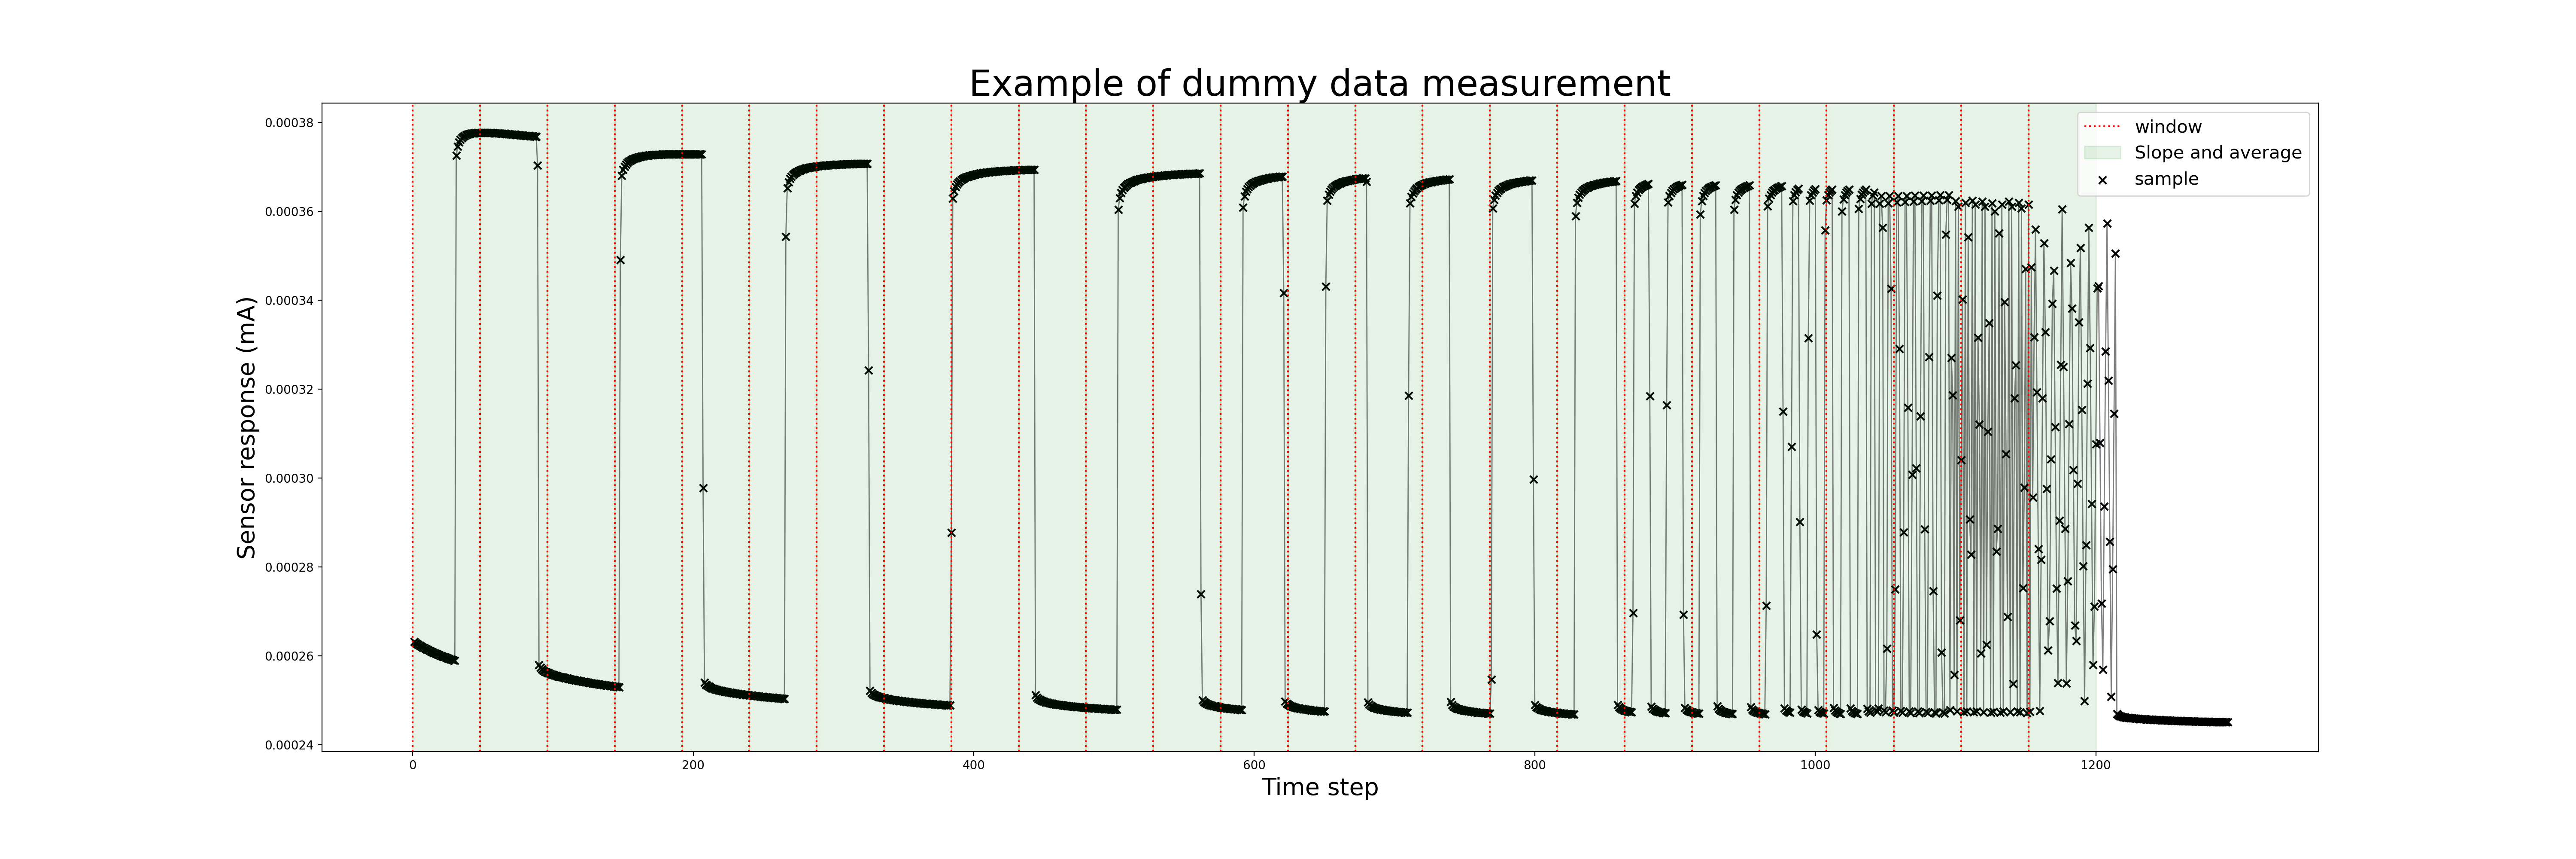
\includegraphics[width=1.2\textwidth]{../../figures/dummy-data.png}
	\end{figure} 

\end{frame}

\begin{frame}
	\frametitle{(Dummy) data}
	
	\begin{figure}[!htb]
		\centering
		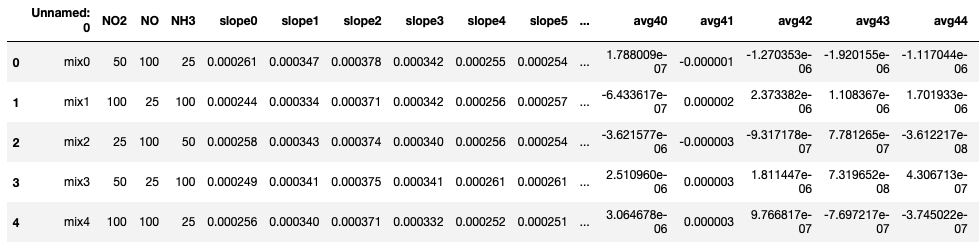
\includegraphics[width=1\textwidth]{../../figures/dummy-feats.png}
	\end{figure} 
	
 	\end{frame}

\begin{frame}
	\section{Methods}
	\frametitle{Methods}
	
	\begin{enumerate}
		\item Linear Regression
		\item Principal Component Regression
		\item Partial Least Squares Regression
		\item Ridge Regression
	\end{enumerate}
	
\end{frame}

\begin{frame}
	\section{(Preliminary) Results}
	\frametitle{(Preliminary) Results}
\end{frame}

\begin{frame}
	\section{Real data}
	\frametitle{Real data will be much better!}
	
	\begin{itemize}
		\item More gas mixtures
		\item More frequencies
		\item More cycles
		\item Shape features directly measured
		\end{itemize}
	
\end{frame}

\begin{frame}
	\frametitle{Real data will be much better!}
	
	\begin{table}[h]
		\centering
		\caption{Data acquisition details}
		\label{tab:measurements}
		\begin{tabular}{|c|c|}
			\hline
			\textbf{Parameter} & \textbf{Value} \\
			\hline
			Factors (gases) & 3 \\
			\hline
			Levels (concentrations) & 5 \\
			\hline
			Frequencies & 16 \\
			\hline
			Features per frequency & 4 (2 slopes and 2 averages) \\
			\hline
			Features per cycle & 64 \\
			\hline
			Number of cycles & 5 \\
			\hline
			Data points per mixture & 320 \\
			\hline
			Number of mixtures & 125 \\
			\hline
			Datapoints per experiment & 40.000 \\
			\hline
			Number of experiments & 3 \\
			\hline
			Total data points & 120.000 \\
			\hline
		\end{tabular}
	\end{table}

\end{frame}

\begin{frame}
	
	\frametitle{Real data will be much better!}

	\begin{figure}[!htb]
		\centering
		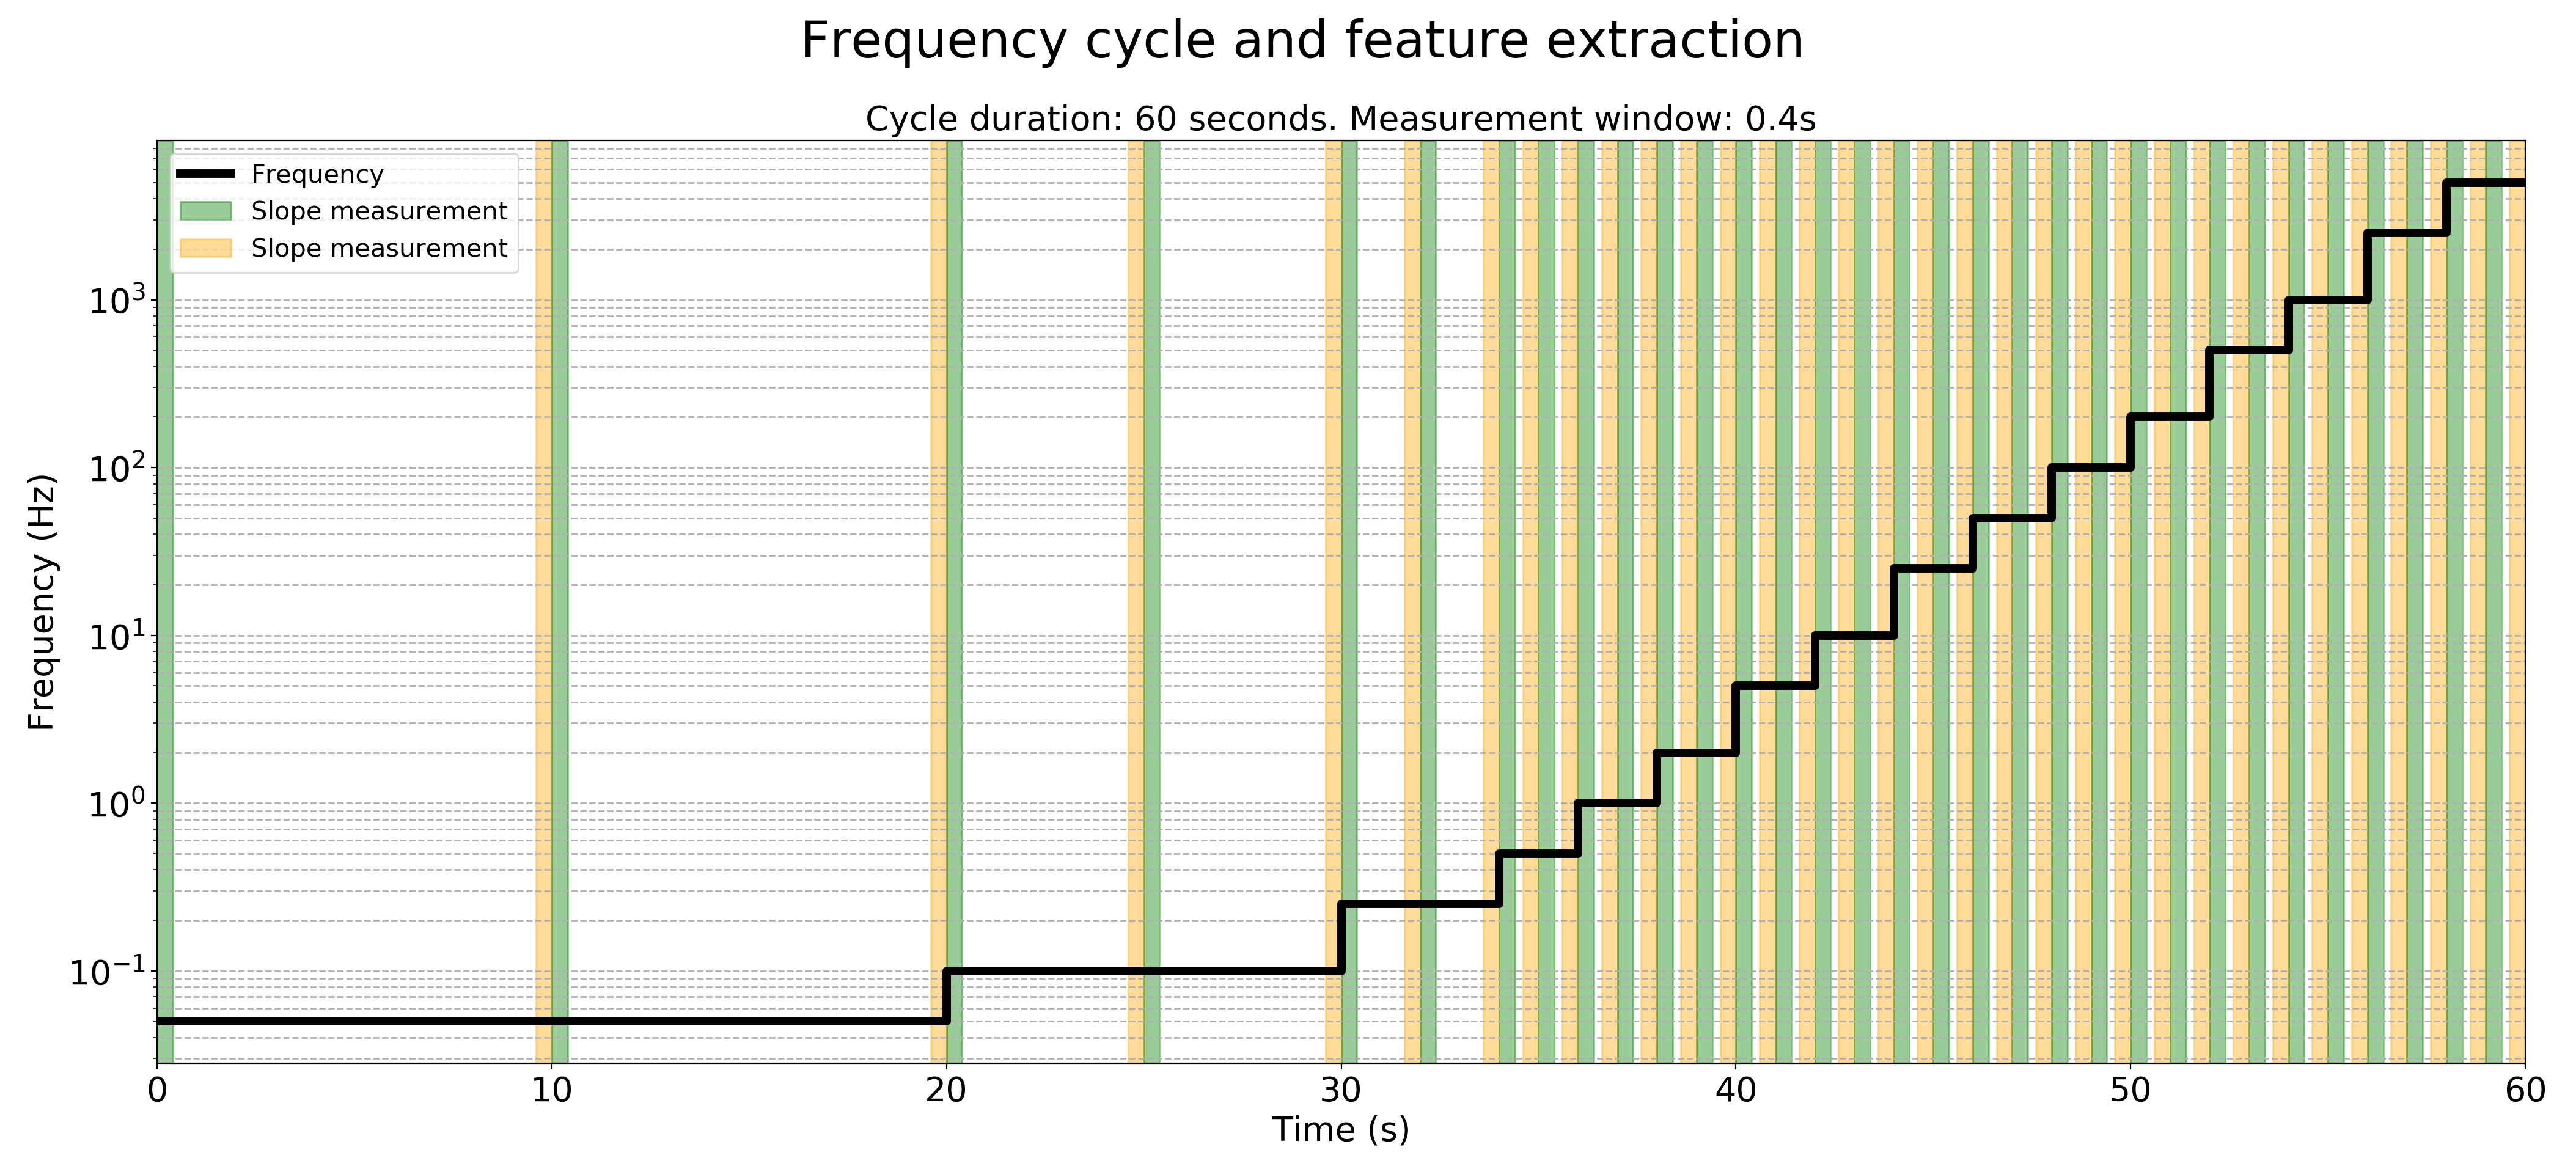
\includegraphics[width=1\textwidth]{../../figures/measurement-windows.png}
		\label{fig:feat-window}
	\end{figure} 
	
\end{frame}

\section{What is next}
\begin{frame}
	\frametitle{What is next}
	\begin{enumerate}
		\item Apply methods to real data
		\item Assess results
		\item Define what is  "good" in "good prediction levels"
		\item Look into neural networks alternatives
		\item Keep writing!
	\end{enumerate}
\end{frame}

\begin{frame}{}
	\centering \Huge
	\emph{Thank you!}
\end{frame}

\end{document}

